Our emphasis in this work is on Latin America.
Protest is an important topic of study in this
region, as many countries here are democracies struggling to consolidate themselves.
The combination of weak channels of communication between citizen and government, and a citizenry that still 
has not grasped the desirability of elections as the means to affect politics means that public protest 
will be an especially attractive option. To illustrate the power of protest in Latin America we need 
only recall that between 1985 and 2011, 17 presidents resigned or were impeached under pressure from 
demonstrations, usually violent, in the streets. Protests have also resulted 
in the rollback of price increases for public services, such as during the `Brazilian Spring' of June 2013.
\begin{figure}
    \centering
    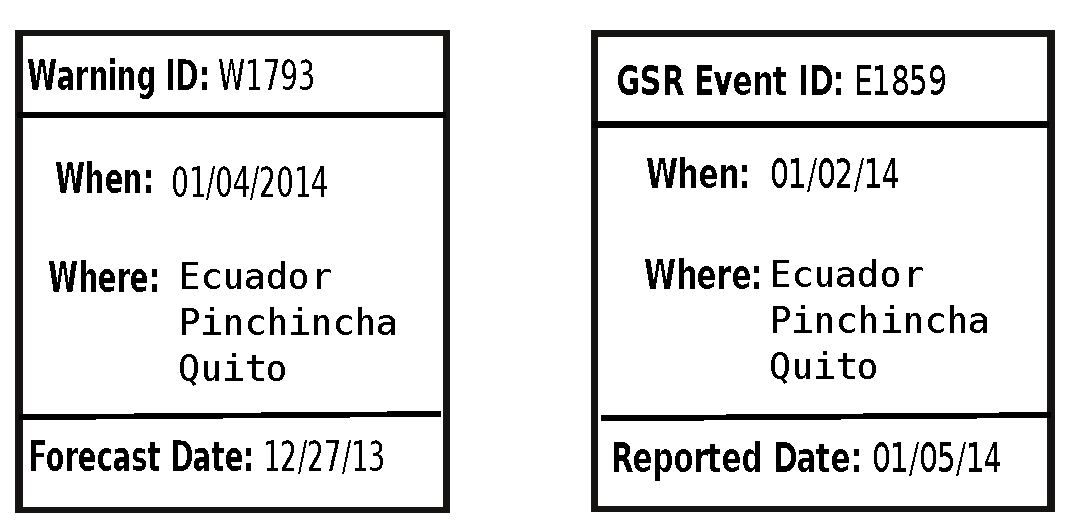
\includegraphics[scale=0.5]{alertstructure}
    \caption{An example warning (left) and GSR event (right).}
    \label{fig:alertstructure}
\end{figure}
Our goal is to identify calls for protests, strikes, or civil disobedience movements from news, blogs, Tweets, and Facebook
pages, with a view toward predicting the {\bf when} (date of the event) and {\bf where}, i.e.,
event location, up to city-level resolution, e.g., 
the city of {\it Tegucigalpa} in the state of {\it Francisco Morazan} in the country of {\it Honduras}).
\iffalse
In addition we seek to forecast the `why' and `who' of the protest.
The {\bf why} (or event type)
captures the main objective or reason for a civil unrest event,
and is meant to come from 7 broad classes (e.g., `Employment \& Wages',
`Housing', `Energy \& Resources' etc.) each of which is further categorized into
whether the event is forecast to be violent or not.
Finally, the {\bf who} (or population)
denotes common categories of human populations
used in event coding~\cite{philschrodt}
such as
Business, Ethnic, Legal (e.g. judges or lawyers), Education (e.g. teachers or students or parents of students), Religious (e.g. clergy), Medical (e.g., doctors or nurses), Media, Labor, Refugees/Displaced, Agricultural (e.g. farmers,
or just General Population. 
\fi
We refer to our forecasts as alerts or warnings (see Fig.~\ref{fig:alertstructure} (left)).
In looking at the structure of the alert, it is important to distinguish between the forecast date (when the forecast is made)
and the predicted event date (i.e., the {\bf when} of the event).


%Concomitant with the definitions in the above section, a GSR event contains
%again the where/why/when/\hskip0ex who of a protest that has actually occurred and
%a {\it reported date} (the date a newspaper reports the protest as
%having happened).
%See Fig.~\ref{fig:alertstructure} (right).
%The GSR is organized by an
%independent third party (MITRE) and the authors of this study do not
%have any participation in this activity. 
\section{Evaluation Metrics -- Quality score}
To evaluate our alerts we have access to a database of protests organized by a third party (source and reference
not provided due to double blind reviewing considerations, but will be added later). We refer to this database as the
GSR (for Gold Standard Report). Human analysts scan newspapers of record in the countries of interest and catalog
protests. The structure of a GSR event (see Fig.~\ref{fig:alertstructure} (right)) is similar to that of an alert with
the only difference being that an event record captures both the reported date (i.e., the date of newspaper publication)
and the event date (i.e., when the newspaper article reports the protest as having happened).
The GSR is available from Nov 2012 
and is used in this paper primarily to 
help evaluate the performance of our system. A manual examination of GSR (as mentioned in Section~\ref{intro}) revealed
that over 75\% of the protests were organized and had clear triggering circumstances with political entrepreneurs leading the
charge to protest.

\subsection{Lead Time vs Accuracy of Forecast Date}
It is important to understand which alerts {\it can} be matched to specific events.
Note that there are four dates in an (alert,event) combination (see Fig.~\ref{fig:timeline}):
\begin{enumerate}
\item The date the forecast is made ({\it forecast date})
\item The date the event is predicted to happen ({\it predicted event date})
\item The date the event actually happens ({\it event date})
\item The date the event is reported in a GSR source ({\it reported date})
\end{enumerate}

\begin{figure}[t]
\centering
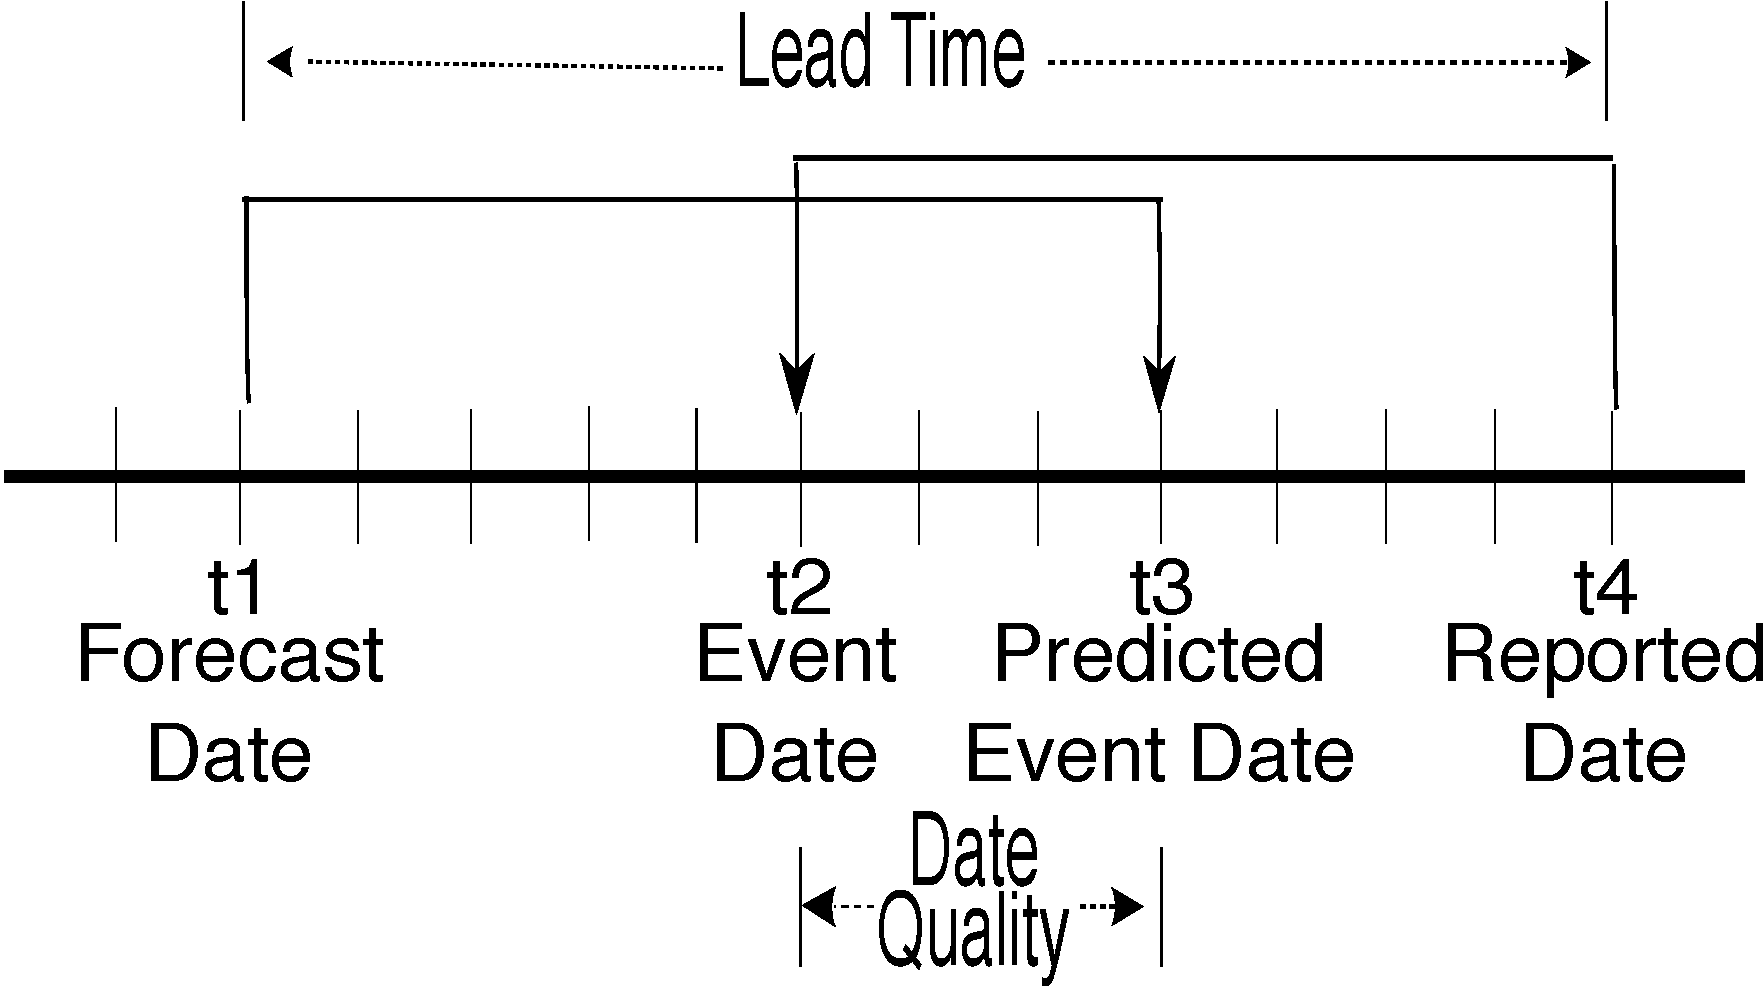
\includegraphics[width=0.40\textwidth]{figures/timeline}
\caption[Timeline depicting lead-time vs date accuracy]{Alert sent at time $t1$ predicting an event at time $t3$
can be matched to a GSR event that happened at time $t2$ and reported
at time $t4$ if $t1 < t4$.}
\label{fig:timeline}
\end{figure}

For an event to be qualified as having been predicted by a warning,
{\it forecast date} $<$ {\it reported date}
(recall that time is measured in
granularities of days).
The {\it lead time} is given as
$(\textit{reported date} - \textit{forecast date})$, i.e., the number
of days by which we `beat the news.'
In constrast, the difference between
{\it predicted event date} and {\it event date}, i.e.,
$|\textit{event date} - \textit{predicted event date}|$.
is one of {\it quality} or accuracy.
Ideally we require {\it lead time} to be as high as possible and
$|\textit{event date} - \textit{predicted event date}|$ to be as low
as possible.

\subsection{Other Quality Aspects}
Forecasting the event date accurately is only one aspect of quality.
Recall that alerts also forecast the location. A scoring formula is also defined for the location quality and 
overall quality score is defined as a sum over both the date and location scores.
$$\textrm{Quality score } (QS) = (DS + LS)*2$$
where DS and LS denote the date score and location score, respectively.
Each of these scores is in turn defined next:
$$DS = 1 - \min(|\textit{event date} - \textit{predicted event date}|,7)/7$$
If the date of the event listed in the warning is the same as the
actual date of the event, then $DS$ is 1. On the other hand, if these dates
are farther than 7 days apart, then $DS$ is 0.

Location score (LS) can be defined in many ways. Because location is
defined in terms of triples of (country, state, city), one approach is
to use a tiered formula. Comparing a GSR event with a warning, we can
obtain a score triple of $(l_1, l_2, l_3)$ where $l_1$ is the
country-level score, $l_2$ is the state-level score, and $l_3$ is the
city-level score. Each of these scores have a value of $0$ if they
do not match and $1$ is they match. Then the match between submitted
warning location and the GSR location is given by:
$$LS = {1 \over 3} l_1 + {1 \over 3} l_1 l_2 + {1 \over 3} l_1 l_2 l_3$$
\noindent
An alternative way to define location score is as:
$$LS = (1 - \min(\textrm{dist},300)/300)$$
where $\textrm{dist}$ denotes the distance (in km) between the city predicted and
the GSR city. All city location names are standardized to the World Gazeteer which provides
latitude and longitude values, thus facilitating the computation of distance.
We use the physical distance based criteria for our purposes.

\subsection{Inclusion Criteria}
Thus far we have demonstrated, given a warning-event pair, how we can
score their fitness. Inclusion criteria define which W-E pairs {\it can}
even be considered for scoring. We have already mentioned one inclusion
criterion, viz. that lead time must be $> 0$. The full list of inclusion
criteria we will consider are:
\begin{enumerate}
\item Lead time $> 0$
\item Both warning and event are for the same country.
\item The {\it predicted event date} and {\it event date} must be
within 7 days of each other.
\end{enumerate}
A fourth, optional (and stringent), criterion we will use is:
%\narenc{Patrick, fix the below enumerate so that it starts at 4.} done
\begin{enumerate}
  \setcounter{enumi}{3}
  \item Both predicted location and event location must be within 300km of
each other.
\end{enumerate}
It is important to distinguish the inclusion criteria from the scoring
criteria. Inclusion criteria define which W-E pairs are allowable.
Scoring criteria determine, from these allowable W-E pairs, what their
score will be.

\subsection{Matching Alerts to Events}
Thus far we have assumed that we matching an alert to a GSR event. In
practice, the problem is we are given a set of issued alerts  and a set
of GSR events and we must determine the quality of the match: which
alert would correspond to which event? One strategy is to construct
a bipartite graph between the set of alerts and the set of events,
where allowable edges are those that satisfy the inclusion criteria, and
where weights on these allowable edges denote their quality scores.
We then construct
a maximum weighted bipartite matching, e.g., see
Fig.~\ref{fig:matching} (middle). Such matchings are conducted on a monthly basis
with a lookback period to bring in unmatched warnings from the previous month.

\begin{figure}[t]
\centering
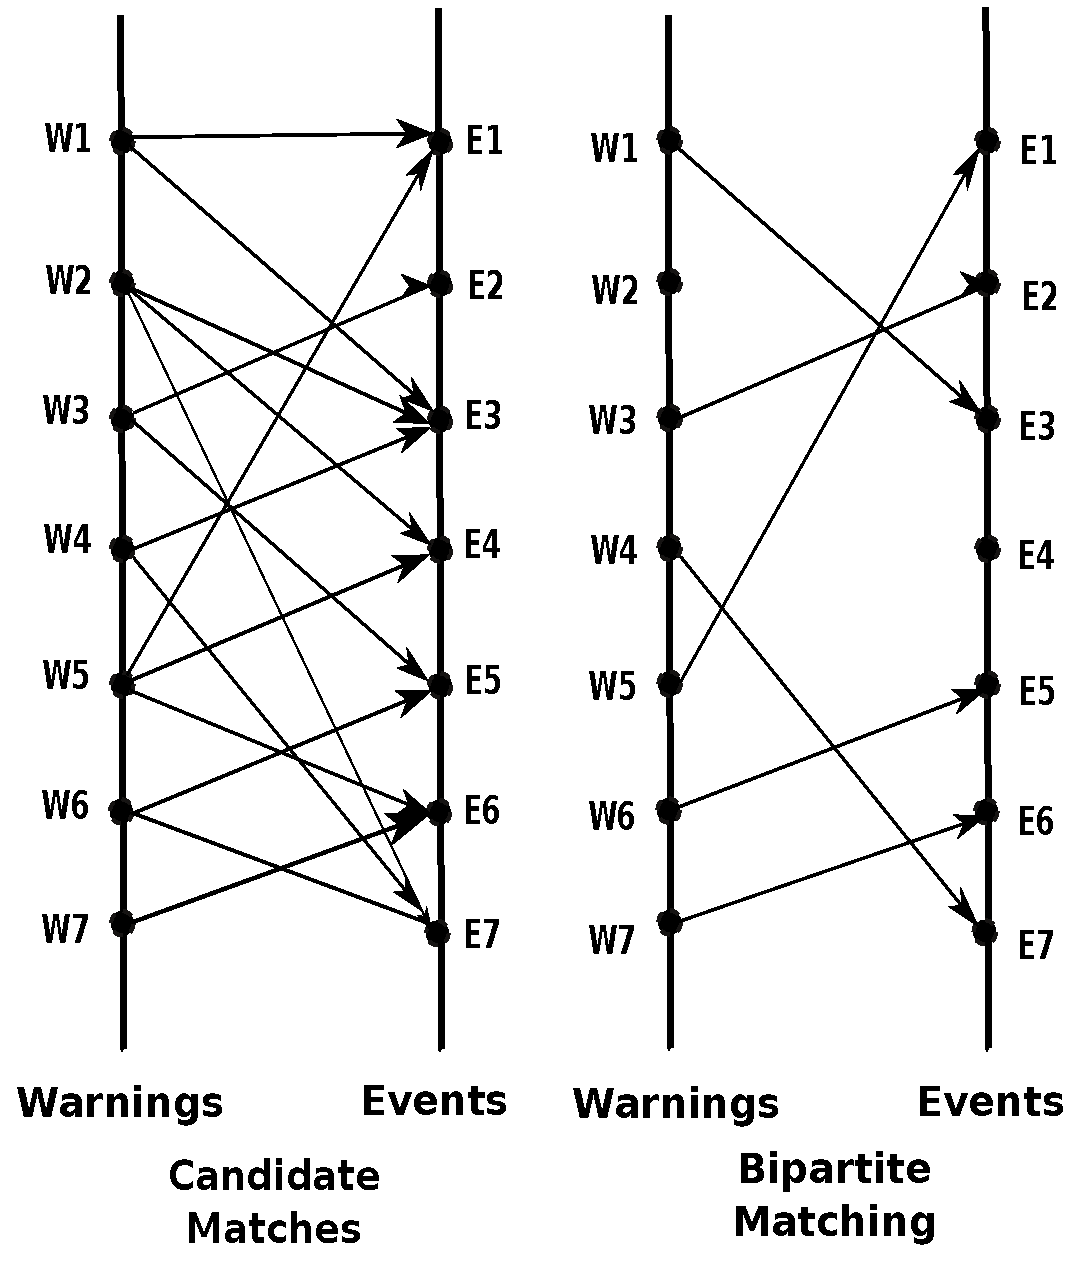
\includegraphics[width=0.50\textwidth]{figures/matching.pdf}
\caption[An example of the bipartite matching used for evaluation]{Given a set of candidate warning-event matches (left), we evaluate the
performance of EMBERS using either a regular bipartite matching (middle) or
by constructing a non-crossing matching (right).}
\label{fig:matching}
\end{figure}


%\subsection{Lead Time vs Accuracy of Forecast Date}
%Before we explain how alerts are matched to events, it is important to
%first understand which alerts {\it can} be matched to specific events.
%Note that there are four dates in an (alert,event) combination (see Fig.~\ref{fig:timeline}):
%\begin{enumerate}
%\item The date the forecast is made ({\it forecast date})
%\item The date the event is predicted to happen ({\it predicted event date})
%\item The date the event actually happens ({\it event date})
%\item The date the event is reported in a GSR source ({\it reported date})
%\end{enumerate}

\iffalse
\subsection{Quality Score}
The Quality score is defined as $$QS = (LS + DS)*2$$ where LS and DS denote location score and date score respectively. The location score is defined based on the kilometre distance between the predicted location and actual location. An alert can be matched to an event, if and only if it is within a 300km radius of the event location. The location score for an alert $Y$ with respect to an event $X$ is defined as $$LS=1 - min(dist(X,Y), 300) / 300 $$
The date score is defined similarly as $$DS = 1 - min( (X-Y), MAXINTERVAL)/MAXINTERVAL$$ where MAXINTERVAL  can be anything. For our experiments, a MAXINTERVAL of 7 days is used. Again a matching cannot occur if $DS=0$
\fi
